\documentclass[unicode,compress,14pt,CJK,aspectratio=169,xcolor={dvipsnames},t%
  \directlua{
    handout = os.getenv"HANDOUT"
    local _ = handout and tex.print(",handout")
}]{beamer}
\usepackage{fontawesome,emoji,amssymb,stmaryrd,scalefnt,relsize}
\usepackage[normalem]{ulem}
\usepackage{luatexja-ruby}
\usepackage{hyperref}
\usepackage{luatexja,luacode}
\usepackage[no-math]{luatexja-fontspec}
\usefonttheme[onlymath]{serif}
\input{../template/beamertemp}
% \setsansfont[Script=Default,Kerning=On,AutoFakeBold,AutoFakeSlant,BoldSlantedFeatures={AutoFakeBold,AutoFakeSlant}]{GenShinGothic-Medium}
\setsansfont[Script=Default, Kerning=On, BoldFont={*-Bold},
ItalicFont={NotoSans-Italic},
Contextuals={Alternate},Ligatures=TeX
]{SourceHanSans}
\setmainfont[Script=Default, Kerning=On, BoldFont={*-Bold},
ItalicFont={NotoSerif-Italic},
Contextuals={Alternate},Ligatures=TeX
]{SourceHanSerif}
\setmainjfont[Script=Default, Kerning=On,
ItalicFont={NotoSerif-Italic},
Renderer=HarfBuzz,
Contextuals={Alternate},Ligatures=TeX
]{SourceHanSerif}
\setsansjfont[Script=Default, Kerning=On, BoldFont={*-Bold},
ItalicFont={NotoSans-Italic}, YokoFeatures={JFM=prop},
Contextuals={Alternate},Ligatures=TeX
]{SourceHanSans}
\newfontfamily{\boldslant}[Script=Default,Kerning=On]{NotoSans-BoldItalic}
\setmonofont[
BoldFont={*-Bold},
ItalicFont={*-Italic},
BoldItalicFont={*-BoldItalic},
Contextuals={Alternate},Ligatures=Common,StylisticSet={1,2,3,4,5,6,7,8,9},Renderer=HarfBuzz]{MonaspiceNeNerdFontMono}
\newjfontfamily{\semijbf}[Script=Default, Kerning=On,
YokoFeatures={JFM=prop}]{SourceHanSans-Medium}
\newfontfamily{\semibf}[Script=Default, Kerning=On, BoldFont={SourceHanSans-Bold},
  BoldItalicFont={NotoSans-BoldItalic},
  ItalicFont={NotoSans-Italic},
]{SourceHanSans-Medium}
\newfontfamily{\osietes}[Script=Default, Kerning=On,
]{Arial Rounded MT Bold}
\renewcommand{\kanjifamilydefault}{\gtdefault}
\usepackage{tikz,pgfplots}
\pgfplotsset{compat=1.18}

\definecolor{accent}{HTML}{2978D6}
\definecolor{basetext}{RGB}{103,103,103}
\definecolor{highlight}{HTML}{D63129}
% \definecolor{subhighlight}{HTML}{2978D6}
\definecolor{subhighlight}{HTML}{0f61b1} % same to titleblue
\definecolor{codebackground}{HTML}{3f3f3f}

\setbeamercolor*{normal text}{fg=basetext}
\setbeamercolor*{section in head/foot}{fg=accent}%
\setbeamercolor*{subsection in head/foot}{fg=accent}%
\setbeamercolor*{headline}{fg=accent}%
\usebeamercolor[fg]{normal text}

\usepackage{minted}
% \usepackage{mdframed}
\usemintedstyle{lovelace}
\setminted{%
  % fontsize=\footnotesize,
  beameroverlays=true,
  frame=single,
  framerule=.08\zw,
  framesep=.6\fboxsep,
  escapeinside=??,
  fontsize=\small,
autogobble}

\newsavebox{\mintedbox}

\usepackage{graphicx}
\usepackage[most]{tcolorbox}
\newtcolorbox{newbie}{
  enhanced,
  boxrule=0pt,
  right skip=0pt,
  left skip=0pt,
  boxsep=0pt,
  right=.3em,
  left=.3em,
  sharp corners,
  colback=black!20,
}
\usetikzlibrary{tikzmark,shapes,arrows,arrows.meta,positioning,calc,fit,shapes.callouts}
\tikzstyle{every picture}+=[line width=1.5pt]
\newcommand{\remembertikz}{\tikz[remember picture]}

% https://tex.stackexchange.com/questions/20425/z-level-in-tikz
\pgfdeclarelayer{1}
\pgfdeclarelayer{2}
\pgfdeclarelayer{3}
\pgfsetlayers{1,2,3,main}
\tikzset{zlevel/.style={%
    execute at begin scope={\pgfonlayer{#1}},
    execute at end scope={\endpgfonlayer}
}}

\tikzset{every picture/.style={remember picture}}
\tikzset{boldarrow/.style={
    arrows={-Triangle[angle=90:10pt]},
    line width=.3\zh
}}
\tikzset{mycallout/.style={
    draw=orange, rectangle callout, rounded corners, outer sep=2pt
}}

% https://tex.stackexchange.com/questions/6135/how-to-make-beamer-overlays-with-tikz-node
\tikzset{onslide/.code args={<#1>#2}{%
    \only<#1>{\pgfkeysalso{#2}}
}}

\newcommand{\itemheader}[1]{%
{\semibf\semijbf #1}}

\usepackage[style=numeric-comp,minalphanames=3,backend=biber]{biblatex}
\renewcommand*{\labelalphaothers}{\textsuperscript{+}}
\renewcommand{\bibfont}{\footnotesize}
\addbibresource{main.bib}
\beamertemplatetextbibitems

\setbeamertemplate{frametitle}{%
  \ifnoframetitle\else%
    \renewcommand{\arraystretch}{0}
    \ifx\insertframesubtitle\empty%
      \begin{beamercolorbox}{frametitle}%
        \vskip-.6\zh\hspace*{-.3\zw}
        \hbox{\large$\blacksquare$ \insertframetitle}\par%
        \raisebox{1.3\baselineskip}[-1pt][2\zh]{%
          \hskip-.06\linewidth\relax%
          \makebox[1.116\linewidth]{%
            \large\mcfamily\bfseries\color{gray!10}%
            \mbox{
              \begin{tabular}{c}
                継\\続
              \end{tabular}
            }
            \hfill
            \mbox{
              \begin{tabular}{c}
                継\\続
              \end{tabular}
        }}}
        \vskip-2.7\zh\hspace*{-.05\linewidth}
        \makebox[1.1\linewidth]{\color{titleblue}\rule{1.1\linewidth}{2pt}}
      \end{beamercolorbox}%
      \vskip-.6\baselineskip
    \else%
      \begin{beamercolorbox}{framesubtitle}%
        \vskip-.6\zh\hspace*{-.3\zw}
        \hbox{{\huge$\bullet$}\large \insertframesubtitle}\par%
        \raisebox{1.3\baselineskip}[-1pt][2.2\zh]{%
          \hskip-.06\linewidth\relax%
          \makebox[1.116\linewidth]{%
            \large\mcfamily\bfseries\color{gray!10}%
            \mbox{
              \begin{tabular}{c}
                継\\続
              \end{tabular}
            }
            \hfill
            \mbox{
              \begin{tabular}{c}
                継\\続
              \end{tabular}
        }}}
        \vskip-2.7\zh\hspace*{-.05\linewidth}
        \makebox[1.1\linewidth]{\color{titleblue!85!}\rule{1.1\linewidth}{2pt}}
      \end{beamercolorbox}
      \vskip-.6\baselineskip
    \fi%
  \fi
}

\newsavebox{\sectionnumberbox}
\setbeamertemplate{section in toc}{%
  \leavevmode%
  \color{titleblue}%
  \savebox{\sectionnumberbox}{\underline{$\blacksquare$ \inserttocsectionnumber.}}
  \usebox{\sectionnumberbox}
  \parbox[t]{\columnwidth-\leftskip-1em-\wd\sectionnumberbox\relax}{%
    \raggedright
    \setlength{\baselineskip}{9pt}
    \inserttocsection
  }
  \par
}
\setbeamertemplate{subsection in toc}{%
  \leavevmode%
  \savebox{\sectionnumberbox}{\underline{$\blacksquare$ \inserttocsectionnumber.}\ }%
  \parbox[t]{\wd\sectionnumberbox\relax}{\rightline{\Large$\bullet$\hspace*{5pt}}}%
  \parbox[t]{\columnwidth-\leftskip-1em-\wd\sectionnumberbox\relax}{%
    \raggedright
    \setlength{\baselineskip}{6pt}
    \small\inserttocsubsection
  }\par
}

\newsavebox{\keizokutoc}
\savebox{\keizokutoc}{%
  \sloppy
  \Huge\scalefont{1.83}
  \parbox[c][.28\baselineskip][c]{1.24\linewidth}{
    \makebox[\linewidth]{\mcfamily\bfseries\color{gray!10}継 \hfill 続}
  }
}

\renewcommand{\TableOfContents}[1]{
    \switchfooter%
    \begin{frame}<beamer>%
      \sloppy
      \centering

      \hspace*{-.09\linewidth}\usebox{\keizokutoc}\par
      \vskip-\dimexpr\ht\keizokutoc+\dp\keizokutoc+.3\baselineskip\relax
      \begin{tabular}[c]{c}
        \textcolor{titleblue}{\tt\Large{}Continuations:}\\
        \rm\large{}continued and to be continued
      \end{tabular}\par
      % \vspace*{-.3\zh}
      \hspace*{-.05\linewidth}
      \makebox[1.1\linewidth]{\color{titleblue}\rule{1.1\linewidth}{2pt}}

      \setlength\columnsep{.5\zw}
      \begin{multicols}{2}%
        \tableofcontents[sectionstyle=show/shaded,subsectionstyle=show/shaded,#1]%
      \end{multicols}%
    \end{frame}%
    \switchfooter}

\AtBeginSection{}
\AtBeginSubsection{}

\title{Continuations: continued and to be continued}
\author{Satoru Kawahara}
\date{June 14, 2025}
\institute{関数型まつり2025}

\begin{document}
\makeatletter
\setbeamertemplate{title page}{
	\begin{center}
		\newsavebox{\keizokutitle}
		\savebox{\keizokutitle}{%
			\parbox[c][.70\textheight][c]{1\linewidth}{%
				\makebox[\linewidth]{\Huge\scalefont{8.5}\mcfamily\bfseries\color{gray!5}継 続}
			}
		}
		\usebox{\keizokutitle}
		\vskip-\dimexpr\ht\keizokutitle+\dp\keizokutitle+1.5\baselineskip\relax

		{
		\Huge
		\hphantom{.}
		\hspace{-.75\zw}%
		\textcolor{green!50!black}{\semibf\scalefont{1.09}C}%
		\kern-.15\zw%
		\textcolor{basetext!50}{\scalefont{1.18}\texttt{[}}%
		\kern-.38\zw%
		\textcolor{black!80!green}{\raisebox{.065\zh}{\texttt{{\scalefont{1.03}o}\kern-2pt n\kern-3pt t\kern-2pt i\kern-4pt n\kern-2pt u\kern-2pt a\kern-4pt t\kern-2pt i\kern-4pt o\kern-2pt n\kern-2pt s}}}%
		\kern-.36\zw%
		\textcolor{basetext!50}{{\scalefont{1.18}\texttt{]\hspace{-.35\zw}:}}}%
		}
		\rm

		\vspace*{1.48\zh}

		\def\@margin{\hspace*{.4\zw}}
		\textcolor{subhighlight}{\LARGE
			$\underleftarrow{\raisebox{0pt}[.4\zh]{\@margin\textrm{continued}\@margin}}$}

		\vspace*{.2\zh}

		\textcolor{basetext}{\large and}

		\vspace*{.3\zh}

		\textcolor{highlight}{\LARGE
			$\overrightarrow{\raisebox{0pt}[.7\zh]{\@margin\textrm{to be continued}\@margin}}$}
		\vspace*{1.8\zh}

		\makebox[.4\linewidth]{\xhrulefill{titleblue}{1pt}}

		\vspace*{.65\zh}

		\small
		\mcfamily
		\color{basetext}

		\textsc{\textmd{%
				{\footnotesize{}At}
				\href{https://2025.fp-matsuri.org/}{\underline{\insertinstitute}}\hspace{.5\zw} {\small\insertdate}
			}}

		\vspace*{.4\zh}

		\insertauthor
	\end{center}
}
\makeatother
\maketitle


% \section*{Who talks}

\switchfooter
\begin{frame}[c]{Who talks}
	% \frametitlesec

	\begin{itemize}
		\item[\emoji{office}]
		      \itemheader{\href{https://corp.eiicon.net}{eiicon, co.,ltd.}}
		\item[\textcolor{gray}{\faicon{paperclip}}] {\small
		      \href{https://twitter.com/Nymphium}{\textcolor{blue!60!white}{\faicon{twitter}}}
		      \href{https://github.com/Nymphium}{\textcolor{black}{\faicon{github}}}
		      Nymphium}\tikzmark{item1}
		\item[\emoji{heart}] OCaml
		\item[\emoji{nerd-face}] Interested in:
		      {\small %
		      \begin{itemize}
			      \item Programming language theory and implementations
			      \item Control-flow and its operators
		      \end{itemize}}

		\item[\emoji{flexed-biceps}]<2-> Motto:

		      \begin{center}
			      {\small\hspace{-2.4\zw}%
				      継続は力なり}

			      \hspace{-2\zw}%
			      \boldslant%
			      {\LARGE{}Continuation is power}

		      \end{center}

	\end{itemize}

	\begin{tikzpicture}[remember picture, overlay]
		\node[anchor = west] (img) at ([xshift=4\zw,yshift=-1.2\zh]pic cs:item1)
		{
\includegraphics[height=5\zh]{img/yh.png}};
		\node[draw,fill=white, ellipse callout, right = .6 of img, callout
		absolute pointer={($(img.east)+(-.2,.2) $)}, xshift=-1\zw,
		yshift=2\zh, align=center] {こんにちは、\\びしょ〜じょです。};
	\end{tikzpicture}
\end{frame}
\switchfooter


\section{Today's Topic}
\begin{frame}
  \frametitlesec

  By the way, do you...

  \large
  \begin{itemize}[<+->]
    \pause
    \item[\emoji{woman-raising-hand}] Use Go Compiler?

    \item[\large \emoji{woman-raising-hand}] {\large Use Optimization?}

    \item[] Then,

      \onslide<+->{
        \huge\vspace*{0.5\zh}\emoji{woman-raising-hand}\vspace*{-2\zh}
        \begin{center}
          \color{red}
          Use

          Profile-Guilded

          Optimization?
        \end{center}
      }
  \end{itemize}
\end{frame}

\begin{frame}
  \frametitlesec
  \Large
  \semibf

  \centering

  Learn about\pause

  \vspace*{15pt}
  {\scalefont{1.8}\color{red}\textbfslant{Profile-Guilded Optimization}}\pause
  \vspace*{6pt}

  and
  \vspace*{10pt}

  around \textcolor{blue}{\scalefont{1.5}its optimizations}

\end{frame}

\section{The Evolution of Continuations}
\TableOfContents{}

\subsection{Dump and J operator, SECD machine}
\begin{frame}[fragile]
	\frametitlesubs

	The first abstract machine for evaluating \textcolor{subhighlight}{functional} programs\cite{landin1964mechanical}:

	\only<.(3)->\small
	\vspace{-.4\zh}
	\begin{table}[h!]
		\begin{tabular}{lcl}

			{\boldslant S}\texttt{tack}                   & : & Stores \underline{intermediate results}                                                \\
			{\boldslant E}\texttt{nvironment}             & : & Stores \underline{variables}                                                           \\
			{\boldslant C}\texttt{ontrol}                 & : & Stores \underline{the next instruction}                                                \\

			\only<.(3)->\large {\boldslant D}\texttt{ump} & : & Stores {\only<.(3)->{\large\bf\color{highlight}}\underline{the suspended computation}} \\
		\end{tabular}
	\end{table}

	\pause
	\vspace{-.4\zh}
	\hspace{1.7\zw}
	And
	\only<.(2)->\large
	\verb|J| operator
		{\only<.(2)->{\bf\color{highlight}}
			captures the \verb|Dump|}\cite{landin1965generalization}

	\pause
	\vspace{-1.4\zh}
	\begin{figure}[h!]
		\begin{tikzpicture}
			\node[rotate=45] (pointup) {\Large\emoji{backhand-index-pointing-right}};
			\node[below = .01 of pointup, anchor=north] {
				\large
				\emoji{face-with-monocle}
				\begin{tabular}{l}
					This marks the origin \\
					of \textbf{\Large continuations!}\cite{10.1023/A:1010060315625}\cite{danvy2004secd}
				\end{tabular}
			};
		\end{tikzpicture}
	\end{figure}
\end{frame}

\subsection{\texttt{call/cc}: \texttt{goto} Practical}
\begin{frame}[fragile]
	\frametitlesubs

	Operators in Scheme\cite{sussman1975scheme}, notably \mintinline{scheme}|call/cc|\cite{scheme1978revised}\footnote{Short of "call-with-current-continuation"}:

	Captures the current continuation as a first-class value

	\begin{minted}{racket}
    (let {[(x (call/cc (λ (?\large\textcolor{highlight}{κ}?)
                (+ 2 (?\large\textcolor{highlight}{κ}? 4)))))]}
        (+ x 3))
    ; => (let {[x 4]} (+ x 3))
    ; => returns 7
  \end{minted}

	\pause
	\mintinline{scheme}{call/cc} can be used to implement:

	\begin{minipage}{.3\textwidth}
		\begin{itemize}
			\item[\emoji{check-mark-button}] non-local exit
			\item[\emoji{check-mark-button}] backtracking
			\item[] $\cdots\cdots$
		\end{itemize}
	\end{minipage}
	\begin{minipage}{.64\textwidth}
		\pause
		{\Huge \emoji{backhand-index-pointing-right}}
		\Large
		\parbox{.85\textwidth}{%
			\color{highlight}
			\bf
			\centering
			ANYTHING related to

			\boldslant control transfer%
		}
	\end{minipage}
\end{frame}

\subsection{Delimited Continuations}
\begin{frame}[fragile]
	\frametitlesubs

	\begin{minipage}{.09\textwidth}
		\
	\end{minipage}
	\begin{minipage}{.9\textwidth}
		\begin{itemize}
			\item[\textcolor{subhighlight}{Problem}:]
			      \mintinline{scheme}{call/cc} is a powerful control structure, but captures the entire rest of the computation (like \mintinline{c}{goto}!)

		\end{itemize}
	\end{minipage}

	\pause
	\vspace{1\zh}
	\hspace{.2\zw}\textcolor{highlight}{Solution}:

	\centering
	\hspace{-.8\baselineskip}
	\begin{minipage}[t]{.60\textwidth}
		\vspace{.2\zh}
		\centering
		{\Large{}Use}

		\textbf{\large{}Delimited Continuations!}\cite{felleisen1988prompt}

		\begin{itemize}
			\item[\emoji{check-mark-button}] capturing \ruby{\textit{scoped}}{delimited} continuations
			\item[\emoji{check-mark-button}] more structured and composable
		\end{itemize}
	\end{minipage}
	\begin{minipage}[t]{.30\textwidth}
		\begin{figure}[h]
			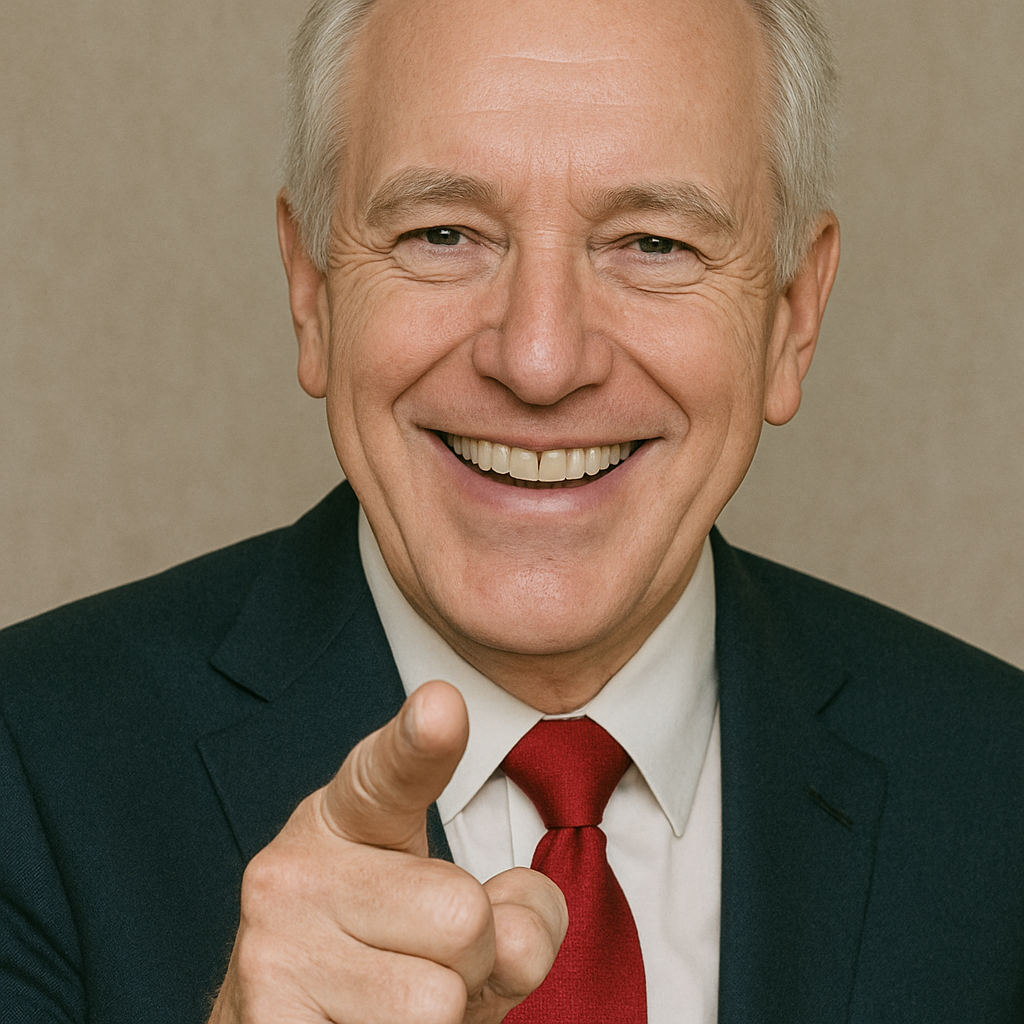
\includegraphics[width=\textwidth]{img/pointing-smile-man.png}
		\end{figure}
	\end{minipage}
\end{frame}

\begin{frame}[fragile]
	\frametitlesubs

	\begin{minted}{racket}
    (+ 3 (reset (+ 4 (shift κ (κ (κ 5))))))

    ; => (+ 3 (+ 4 (+ 4 5)))
  \end{minted}

	\pause
	\begin{minipage}[t]{.49\textwidth}
		Several variants of operators:
		\only<.(2)->{\raisebox{-.2\baselineskip}{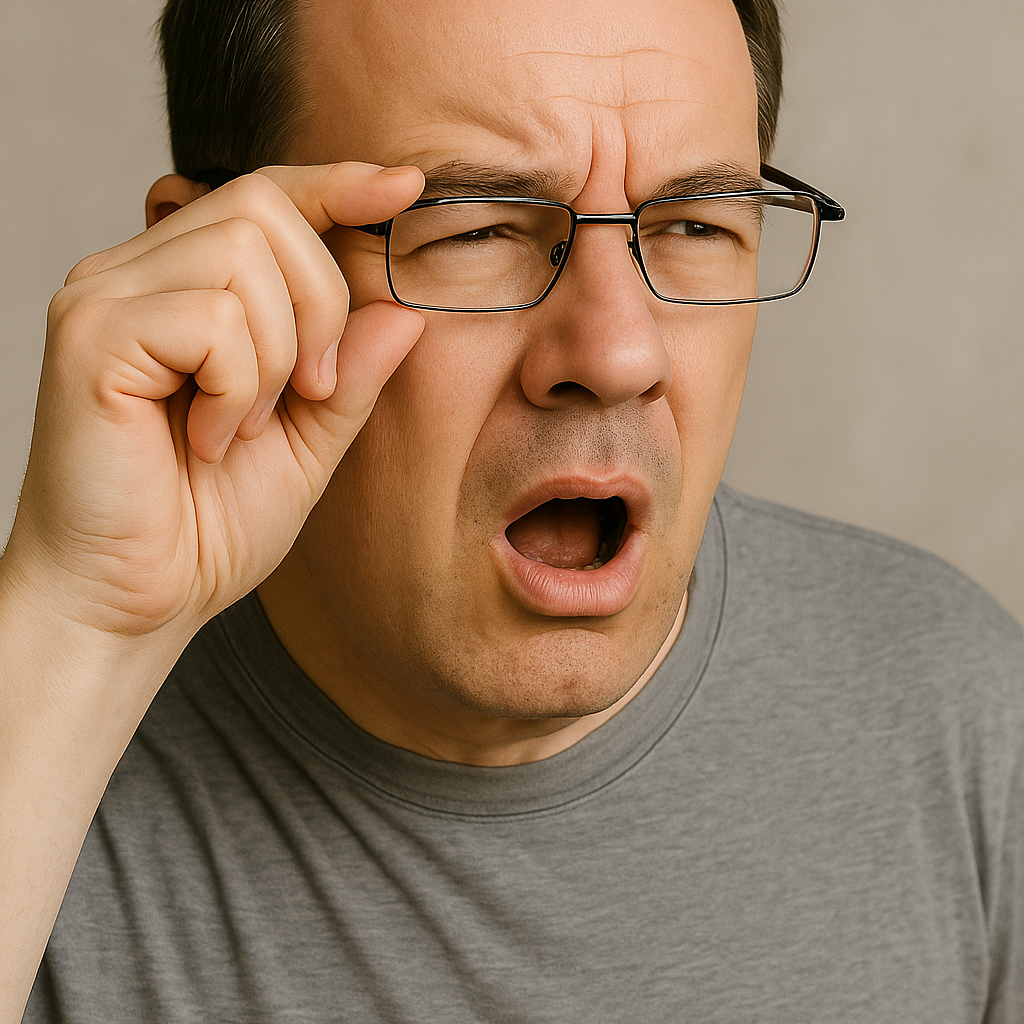
\includegraphics[width=.9\baselineskip]{img/gaze.png}}\vskip2\baselineskip}

		\only<.(1)>{\centerline{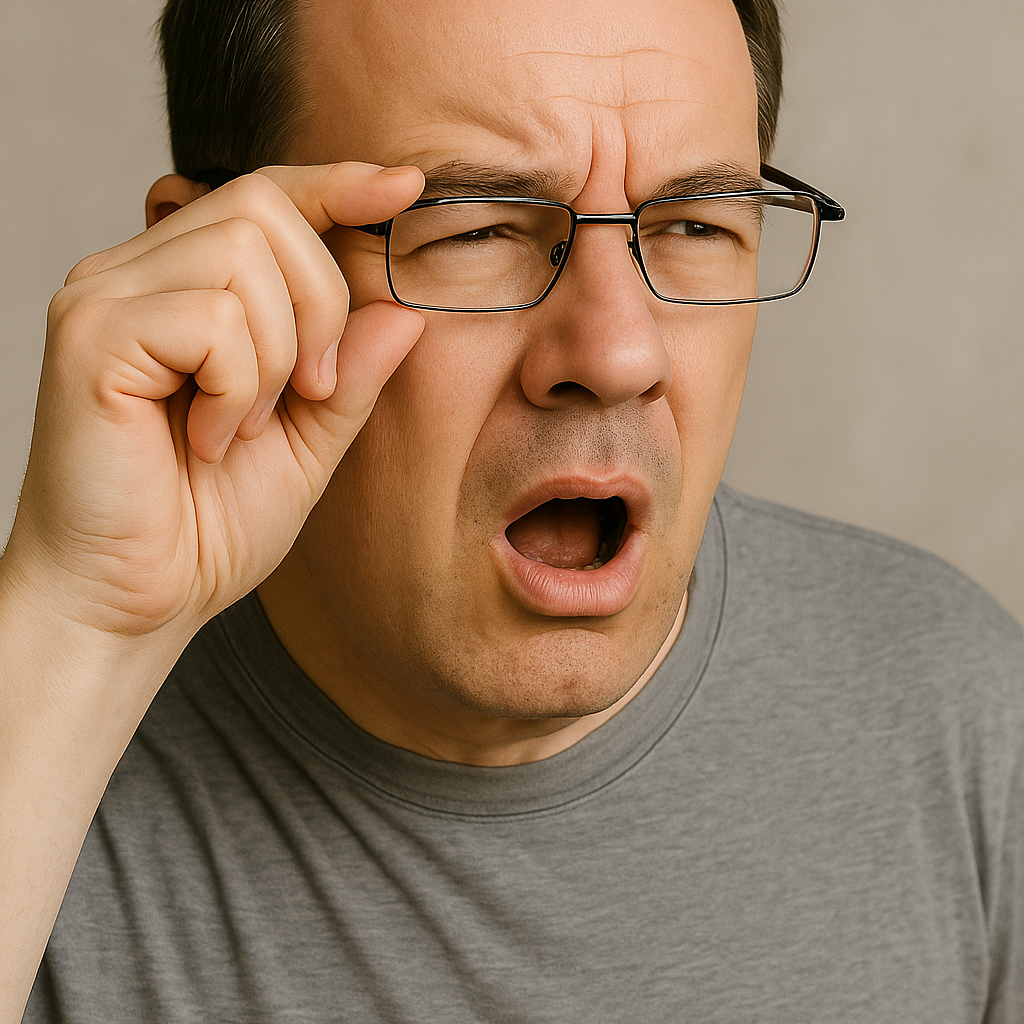
\includegraphics[width=7\baselineskip]{img/gaze.png}}}
	\end{minipage}
	\begin{minipage}[t]{10\zw}
		\alt<.(1)>{\vskip-.8\baselineskip\footnotesize}{\scriptsize}
		\begin{tabular}{l}
			$\bullet$ \texttt{control/prompt}\cite{felleisen1988prompt} $\texttt{control}_0\texttt{/}\texttt{prompt}_0$\cite{shan2004shift} \\
			$\bullet$ \texttt{shift/reset}\cite{danvy1990abstracting} $\texttt{shift}_0\texttt{/}\texttt{reset}_0$\cite{shan2004shift}      \\
			$\bullet$ \texttt{fcontrol/run}\cite{Dorai1993handling}                                                                         \\
			$\bullet$ \textit{multiprompt} extensions\cite{dybvig2005a}                                                                     \\
			$\bullet$ $\cdots\cdots$
		\end{tabular}
		\only<.(2)->{\vskip.8\baselineskip}
	\end{minipage}

	\pause
	Delimited continuations enable us to implement

	\begin{minipage}[c]{.35\textwidth}
		\begin{itemize}
			\item[\emoji{check-mark-button}] \mintinline[fontsize=\large]{scheme}|call/cc|\textbf{!}
			\item[\emoji{check-mark-button}] \textcolor{subhighlight}{\bf ALL \underline{monads}!!}
		\end{itemize}
	\end{minipage}
	\pause
	\begin{minipage}[c]{.64\textwidth}
		\LARGE
		$\cdots\cdots$and \textcolor{highlight}{\bf vice-versa!}\cite{dybvig2005a}
	\end{minipage}

	\begin{center}
		\begin{tikzpicture}
			\smaller[1]
			\node (callcc) {\texttt{call/cc}};
			\coordinate[below = .9 of callcc] (middle);
			\node[right = .60 of middle] (monads) {monads};
			\node[left = .55 of middle, inner sep =0pt, outer sep = 2pt] (delimcc) {
				\renewcommand{\arraystretch}{0.3}
				\begin{tabular}{c}
					delimited \\
					controls
				\end{tabular}
			};

			\draw[->,thick]
			([xshift=.3\zw]callcc.south) edge (monads.north west)
			(monads.north west) edge node[sloped, above=0] {$\equiv$} ([xshift=.3\zw]callcc.south)

			(monads) edge node[sloped, below=0] {$\equiv$} (delimcc)
			(delimcc) edge (monads)

			(delimcc.north east) edge node[sloped, above=0] {$\equiv$} ([xshift=-.3\zw]callcc.south)
			% TODO: 矢印ねじれ
			([xshift=-.3\zw]callcc.south) edge (delimcc.north east);
		\end{tikzpicture}
	\end{center}
\end{frame}

\subsection{Continuation-Passing Style}
\begin{frame}[fragile]
	\frametitlesubs

	A program representation where control flow is made \textit{\semibf explicit}
	\\by chaining computations as \textcolor{subhighlight}{continuations}\cite{reynolds1972definitional}:

	\def\relanime{4}

	\begin{center}
		\only<.(\relanime)->{%
			\setminted{fontsize=\smaller[2]}\smaller[2]
			\vskip-.8\zh\relax
		}

		\tikzstyle{every picture}+=[remember picture]
		\begin{minipage}[c]{9\zw}
			\begin{minted}{racket}
        (define (add1 x)
          (+ x 1))
        (define (mul2 x)
          (* x 2))

        ?\tikzmarknode{origord2a}?(mul2 ?\tikzmarknode{origord1a}?(add1 3)?\tikzmarknode{origord1}?)?\tikzmarknode{origord2}?
      \end{minted}
		\end{minipage}
		\pause
		\begin{minipage}[c]{6\zw}
			\smaller
			\centering
			\color{highlight}\bf
			CPS\\
			$\underrightarrow{\textsf{Conversion!}}$
		\end{minipage}
		\begin{minipage}[c]{11\zw}
			\begin{minted}{racket}
        (define (add1 x ?\larger\textcolor{highlight}{κ}?)
          (?\larger\textcolor{highlight}{κ}? (+ x 1)))
        (define (mul2 x ?\larger\textcolor{highlight}{κ}?)
          (?\larger\textcolor{highlight}{κ}? (* x 2)))

        ?\tikzmarknode{cpsord1a}?(add1 3?\tikzmarknode{cpsord1}? (λ (smu)
          ?\tikzmarknode{cpsord2a}?(mul2 sum?\tikzmarknode{cpsord2}? (λ (mul)
            mul))))
      \end{minted}
		\end{minipage}
	\end{center}

	\pause{}
	CPS \underline{\textit{fixes}} the order of evaluation and control flow%
	\begin{tikzpicture}[overlay, remember picture, every node/.style={inner sep=0pt}, underline/.style={line width=1pt,draw}]
		% \smaller
		\only<.(1)->{\smaller[2]}
		\node[color=SeaGreen,circle,draw,anchor=south east,yshift=.7\baselineskip] at (origord1) {1};
		\path[underline, color=SeaGreen] ([yshift=-.2\zh]origord1a.north) -- ([yshift=-.2\zh]origord1.north);

		\node[color=Peach,circle,draw,anchor=south east,yshift=.7\baselineskip, xshift=.5\zw] at (origord2) {2};
		\path[underline, color=Peach] ([yshift=-.4\zh]origord2a.north) -- ([yshift=-.4\zh]origord2.north);

		\node[color=SeaGreen,circle,draw,anchor=south east,yshift=.7\baselineskip, xshift=.3\zw] at (cpsord1)  {1};
		\path[underline, color=SeaGreen] ([yshift=-.2\zh]cpsord1a.north) -- ([yshift=-.2\zh]cpsord1.north);

		\node[color=Peach,circle,draw,anchor=north east,yshift=-.2\baselineskip, xshift=.7\zw] at (cpsord2)  {2};
		\path[underline,color=Peach] ([yshift=-.2\zh]cpsord2a.north) -- ([yshift=-.2\zh]cpsord2.north);
	\end{tikzpicture}%
	\pause{},

	so that it's a good choice for

	\centerline{\Large\textbf{an intermediate representation}}

	for language implementations!
\end{frame}

\subsection{Compiling with Continuations}
\begin{frame}[fragile]
	\frametitlesubs

	CPS as \textcolor{subhighlight}{an intermediate representation} (IR) for language impls\cite{appel1992cwc}:

	\begin{center}
		\begin{tikzpicture}
			\smaller[2]
			\node[draw] (src) {Source};
			\node[right = of src,draw] (cps) {\color{highlight}\larger CPS};
			\node[right = 1.8 of cps, draw] (gen) {Codegen};
			\node (opts) at ($(cps.south east)!0.5!(gen.south west)$) {(Opts.)};
			\draw[->,thick]
			(src) edge (cps)
			(cps) edge (gen);
		\end{tikzpicture}
	\end{center}

	\pause
	\begin{itemize}
		\item[\emoji{check-mark-button}]<+->
		      Good for \textcolor{subhighlight}{\bf functional languages}

		      \smaller
		      CPS operates functions as first-class values!
		      \tikz[remember picture, overlay]\node[left = 0.2 of src.west]{
			      \scalebox{.7}{
				      $\left.
					      \begin{array}{l}
						      \textsf{SML/NJ} \\
						      \textsf{Scheme} \\
						      \begin{array}{c}
							      \textsf{OCaml} \\
							      {\scriptsize\left(
							      \begin{array}{c}
									      \textsf{flambda} \\
									      \textsf{wasm}
								      \end{array}
							      \right)}
						      \end{array}
					      \end{array}
					      \right\}$
			      }
		      };

		\item[\emoji{check-mark-button}]<+->
		      Good for \textcolor{subhighlight}{\bf optimizations}

		      \smaller
		      Several optimizations can be done by \textcolor{highlight}{β}/\textcolor{highlight}{η},

		      and each values are single-assignment!
		      \smaller[3]
		      \begin{lrbox}{\mintedbox}
			      \begin{minipage}{14.5\zw}
				      \setminted{fontsize=\relsize{0}}
				      \begin{minted}{OCaml}
                let z = a * b + a * b
                in e
              \end{minted}
			      \end{minipage}
		      \end{lrbox}
		      \begin{tikzpicture}[remember picture, overlay]
			      \node[draw, below right = -.05 of opts, xshift=4\zw] (optmap) {
				      \setlength{\tabcolsep}{.15\zw}
				      \begin{tabular}{c r l}
					      \begin{tabular}{c}
						      Constant Folding \\
						      \& Inlining
					      \end{tabular}
					                          & $\Rightarrow$ & β reduction  \\
					      Defunctionalization & $\Rightarrow$ & η reduction  \\
					      \begin{tabular}{c}
						      Common Subexpression \\
						      Elimination
					      \end{tabular}
					                          & $\Rightarrow$ & \textit{EZ}:
				      \end{tabular}
			      };

			      \node[below = .0 of optmap.south west, anchor=north west] (raw) {\usebox{\mintedbox}};
		      \end{tikzpicture}

		      \begin{lrbox}{\mintedbox}
			      \begin{minipage}{15\zw}
				      \setminted{fontsize=\relsize{0}}
				      \begin{minted}{OCaml}
                ?\tikzmarknode{ab1}{}?( *' ) a b?\tikzmarknode{ab1e}{}? (fun ?$\texttt{v}_1$? ->
                ?\tikzmarknode{ab2}{}?( *' ) a b?\tikzmarknode{ab2e}{}? (fun ?$\texttt{v}_2$? ->
                ( +' ) ?$\texttt{v}_1$? ?$\texttt{v}_2$? (fun z ->
                ?$\llbracket\texttt{e}\rrbracket$?
              \end{minted}
			      \end{minipage}
		      \end{lrbox}
		      \begin{tikzpicture}[remember picture, overlay]
			      \node[below = .0 of raw.south west, anchor=north west] (cpsed) {\usebox{\mintedbox}};
			      \path[draw] (raw.east) edge[bend left=30,->] node[midway,right = 0]{
					      \smaller
					      \begin{tabular}{c}
						      CPS        \\
						      Conversion \\
						      ($\llbracket-\rrbracket$)
					      \end{tabular}
				      }
			      (cpsed.east);

			      \path[draw, line width=0.1\zh,color=highlight]
			      ([yshift=-.2\zw]ab1.south) -- ([yshift=-.2\zw]ab1e.south)
			      ([yshift=-.2\zw]ab2.south) -- ([yshift=-.2\zw]ab2e.south);
			      \node[above= .2 of ab1e.north east,fill=white,opacity=0.5,text opacity=1] {\color{highlight}same!};
		      \end{tikzpicture}
	\end{itemize}
\end{frame}

\subsection{Correspondence between procedural}
\begin{frame}[fragile]
	\frametitlesubs

	How do \textit{control transfers} correspond in \textcolor{highlight}{functional} and \textcolor{subhighlight}{procedural}?

	% TODO: 表にして横にならべる
	\begin{itemize}
		\item Functional side:
		      \begin{itemize}
			      \pause
			      \item<+->[\emoji{down-arrow}] \verb|J|: Low-level continuation operator
			      \item<+->[\emoji{down-arrow}] \verb|call/cc|: Capturing entire continuation
			      \item<+->[\emoji{backhand-index-pointing-right}] \verb|shift/reset|: Structured, modular and composable control
			      \item<+->[\emoji{gear}] {\large \textcolor{highlight}{\textbf{CPS} as an IR}}
		      \end{itemize}

		\item Procedural side:
		      \begin{itemize}
			      \item<.(-5)->[\emoji{down-arrow}] \verb|jmp|: Low-level control transfer\tikzmarknode{pos}{}
			      \item<.(-2)->[\emoji{down-arrow}] \verb|goto|: Arbitrary jumps in high-level repr.
			      \item<.(-1)->[\emoji{backhand-index-pointing-right}] \verb|for| / \verb|while| / \verb|if|: Structured, clear control\cite{dijkstra1972structured}
			      \item<.(0)->[\emoji{gear}] {\large \textcolor{subhighlight}{\textbf{SSA}\footnote{Static Single-Assignment form} as an IR}}\vspace*{-.3\baselineskip}
		      \end{itemize}
	\end{itemize}

	\only<.->{
		\begin{tikzpicture}[overlay]
			\node[right = 3.5\zw of pos,yshift=0.7\zh] (cpsssa) {
				\begin{tabular}{l}
					And also, \\
					{\Large \textbf{\textcolor{highlight}{CPS}} $\Leftrightarrow$ \textbf{\textcolor{subhighlight}{SSA}!} \cite{10.1145/278283.278285}}
				\end{tabular}
			};
		\end{tikzpicture}
	}
\end{frame}

% \addtocontents{toc}{\vfill\newpage} % tocを改行
\section{Continuations with Effects}
\TableOfContents{}

\subsection{Why continuations for effects?}
\begin{frame}
	\frametitlesubs{}

	{
		\only<.(3)->{\smaller[2]}
		\textit{Effects}, side effects or computational effects:
		\vspace*{-1.1\zh}

		\begin{center}
			\begin{minipage}[t]{.7\textwidth}
				\begin{itemize}
					\only<.(3)->{\setlength{\itemsep}{-.2\zh}}
					\item Exception {\only<.(2)->{\dotfill \textit{halt?}}}
					\item Async I/O {\only<.(2)->{\dotfill \textit{when to resume?}}}
					\item Coroutines {\only<.(2)->{\dotfill \textit{which order to resume?}}}
					\item etc.
				\end{itemize}
			\end{minipage}
		\end{center}
	}

	\vspace{.2\zh}
	Handling effects is about what happens------
	\pause
	\\\centerline{\larger{}and \textit{when} and \textit{how} to \textcolor{subhighlight}{resume}.}

	\pause

	\vspace{-.4\zh}
	\centering
	\hspace*{\fill}
	\begin{minipage}[t]{.41\textwidth}
		\vspace{.6\zh}

		\centering
		\large
		So, it's time
		for
		\LARGE
		\textcolor{highlight}{\boldslant Continuations!}
	\end{minipage}
	\begin{minipage}[t]{.30\textwidth}
		\begin{figure}[h]
			\centering
			\sloppy
			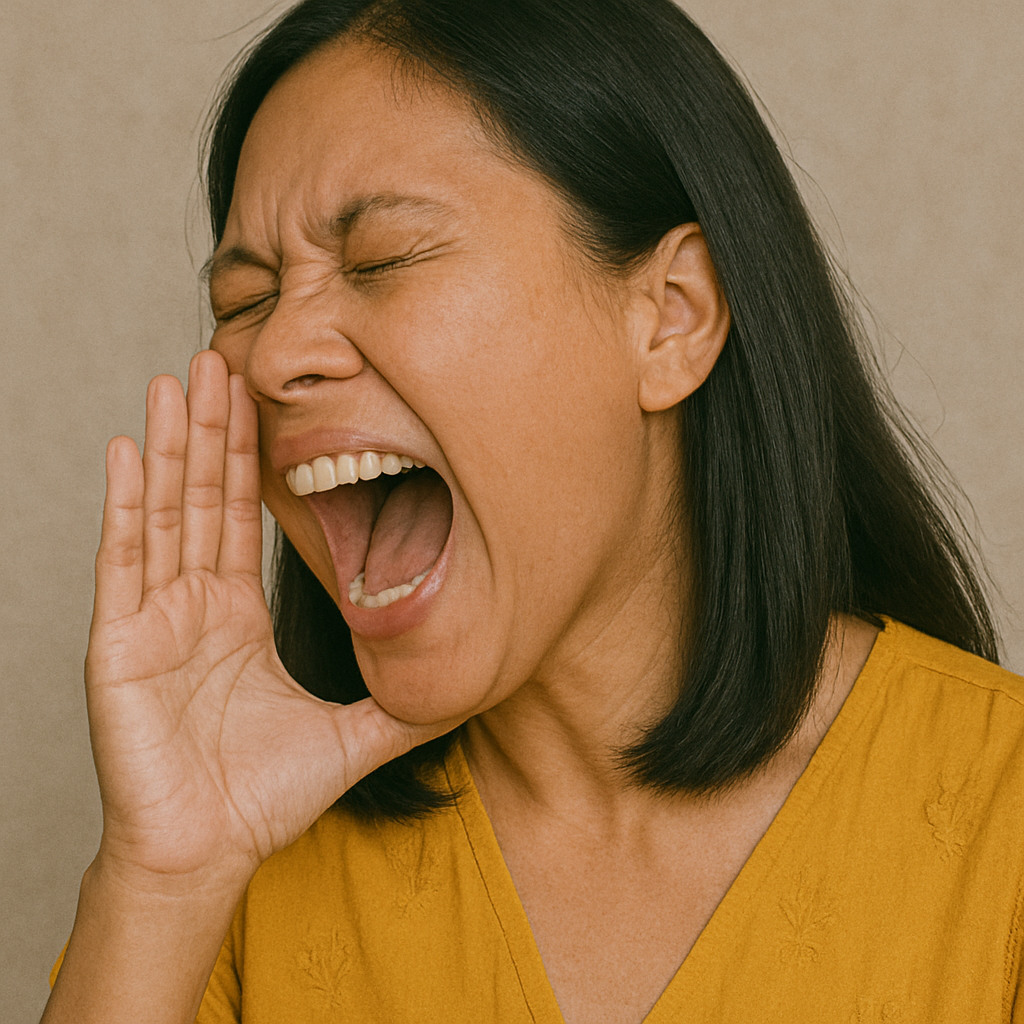
\includegraphics[height=.38\textheight]{img/woman-shouting.png}
		\end{figure}
	\end{minipage}
\end{frame}

\subsection{Monads}

\begin{frame}[fragile]
	\frametitlesubs{}

	An approach to modeling calculi with \textit{effects}\cite{moggi1991notions}:

	\begin{center}
		\begin{minipage}{.63\textwidth}
			\begin{minted}{haskell}
        class Monad m where
          return :: a -> m a
          (>>=)  :: m a -> ?\tikzmarknode{bindk}?(a -> m b) -> m b?\tikzmarknode{bindke}?
      \end{minted}
		\end{minipage}
	\end{center}

	\pause
	\begin{tikzpicture}[overlay]
		\path[draw, line width=1.5pt, color=highlight] ([yshift=-.2\zh]bindk.south) edge node[midway,above=0.4]{\footnotesize continuation} ([yshift=-.2\zh]bindke.south);
	\end{tikzpicture}

	\pause
	\centering

	\setminted{fontsize=\footnotesize}
	\begin{minipage}{.4\textwidth}
		\begin{minted}{haskell}
      instance Monad Maybe where
        return = Just
        Just x  >>= k = k x
        Nothing >>= ?\tikzmarknode{nothing}{\texttt{\_}}? = Nothing
    \end{minted}
	\end{minipage}
	\hspace{.1\textwidth}
	\begin{minipage}{.3\textwidth}
		\pause

		\begin{minted}{haskell}
      maybe e >>= \x -> u
    \end{minted}
		\vskip-.1\baselineskip

		\pause

		\centering
		\begin{tabular}{rl}
			$\Downarrow$ &
			\smaller[2]
			\begin{tabular}{c}
				direct-style \\
				with \texttt{do}
			\end{tabular}
		\end{tabular}
		\vskip-.1\baselineskip

		\begin{minipage}{.75\textwidth}
			\begin{minted}{haskell}
        do
          x <- maybe e
          u
      \end{minted}
		\end{minipage}
	\end{minipage}

	\pause

	\begin{tikzpicture}[overlay]
		\node at (nothing) {\LARGE\textcolor{highlight}{\bf\_}};
		\node[below = .2 of nothing, rotate=-20] {\Huge\emoji{backhand-index-pointing-up}};
		\node[below right = .2 of nothing, yshift=-.7\baselineskip] {
			\small
			\begin{tabular}{l}
				\textcolor{highlight}{throw away} continuation \\
				to stop computation\textbf{!}
			\end{tabular}
		};
	\end{tikzpicture}
\end{frame}

\subsection{Algebraic Effect Handlers}
\begin{frame}[fragile]
	\frametitlesubs

	A new way to model effectful computations, with high \textit{modularity} and \textit{composablility}\cite{bauer2013effect}:

	\vskip-.2\baselineskip
	\begin{center}
		\begin{minipage}{.7\textwidth}
			\begin{minted}{ocaml}
        type _ eff += Print : string -> unit eff

        match perform @@ Print "hello" with
        | effect (Print msg), ?\textcolor{highlight}{\bf\tt k}? ->
          print_endline msg; ?\textcolor{highlight}{\bf\tt continue k ()}?
      \end{minted}
		\end{minipage}
	\end{center}

	\pause

	\begin{center}
		\vspace*{-.1\baselineskip}
		\begin{minipage}[t]{.44\textwidth}
			\centering
			\parbox[c][.35\textheight][c]{\textwidth}{
				\begin{center}
					\textcolor{subhighlight}{Handlers} make it \textit{easier} to \textbf{compose} and \textbf{modularise}

					than

					\textcolor{highlight}{monad transformers}\textbf{!}
				\end{center}
			}
		\end{minipage}
		\hspace{.03\textwidth}
		\begin{minipage}[t]{.4\textwidth}
			\parbox[t][.3\textheight][t]{\textwidth}{
				
\includegraphics[width=3.6\zw]{img/notgood.png}\raisebox{2\zh}{\tiny\footnote{\url{https://www.youtube.com/watch?v=uxpDa-c-4Mc}}}
				\raisebox{1.2\baselineskip}{\mbox{
						\footnotesize
						\color{highlight}
						\begin{tabular}{c}
							Monad \\
							Transformers
						\end{tabular}
					}}
				\vskip-.4\baselineskip

				
\includegraphics[width=3.6\zw]{img/good.png}
				\raisebox{\baselineskip}{\mbox{
						\footnotesize
						\color{subhighlight}
						\begin{tabular}{c}
							Algebraic Effect \\
							Handlers
						\end{tabular}
					}}}
		\end{minipage}
	\end{center}
\end{frame}

% \section{Type Systems with Continuations}

\begin{frame}
	\frametitlesec

	\begin{itemize}
		\item Linear types for continuations
		\item Answer-Type Modification
	\end{itemize}
\end{frame}

% 

\section{まとめ}
\begin{frame}
    \frametitlesec

    \begin{itemize}
        \item[\coloremoji{🌋}] Algebraic Effectsが楽しい

            ICFP 2018やML Workshop2018にも\\
            AE関連のトピック%
            \footnote{\url{https://icfp18.sigplan.org/event/mlfamilyworkshop-2018-papers-programming-with-abstract-algebraic-effects}}%
            \footnote{\url{https://icfp18.sigplan.org/event/icfp-2018-papers-versatile-event-correlation-with-algebraic-effects}}

        \item[\coloremoji{🉐}] Algebraic Effects使おう

            \begin{itemize}
                \item[\coloremoji{🛠}] インプリいろいろ
                \item[\coloremoji{💪}] なければ自作も可
            \end{itemize}

        \item[\coloremoji{👨‍💻}] 研究やってます
    \end{itemize}
\end{frame}



\switchfooter
\begin{frame}[allowframebreaks]{References}
	\printbibliography
\end{frame}
\end{document}
